\documentclass[11pt,a4paper]{article}
\usepackage[utf8]{inputenc}
\usepackage[vietnamese]{babel}
\usepackage{amsmath,amssymb}
\usepackage[version=4]{mhchem}
\usepackage{geometry}
\geometry{top=1.5cm,bottom=1.2cm,left=1.4cm,right=1.4cm,headheight=28pt,headsep=12pt,footskip=18pt}
\usepackage{graphicx}
\usepackage{xcolor}
\usepackage{tabularx}
\usepackage{array}
\usepackage{tikz}
\usepackage{multicol}
\usepackage{fancyhdr}
\usepackage{enumitem}

\definecolor{hfRed}{HTML}{D32F2F}
\definecolor{hfGreen}{HTML}{8BC390}
\definecolor{mainGreen}{HTML}{2E7D32}

\usepackage{ex_test}
\bracketExpl{true}

\pagestyle{fancy}
\fancyhf{}
\renewcommand{\headrulewidth}{0.75pt}
\renewcommand{\headrule}{\hbox to\headwidth{\color{hfGreen}\leaders\hrule height \headrulewidth\hfill}}
\renewcommand{\footrulewidth}{0.75pt}
\renewcommand{\footrule}{\hbox to\headwidth{\color{hfGreen}\leaders\hrule height \footrulewidth\hfill}}

\fancyhead[L]{\small\itshape\color{hfRed}Tài liệu lưu hành nội bộ}
\fancyhead[R]{\small\color{hfRed}Thầy \textbf{TRẦN VĂN THẠNH} - 0777.470.803}

\fancyfoot[L]{\footnotesize\itshape\color{hfRed}CS1: 6/15 Nguyễn Hoàng, P. Kim Long, TP Huế \quad|\quad CS2: 24 Đặng Thái Thân, TP Huế}
\fancyfoot[R]{\small\textbf{\color{hfRed}Trang \thepage}}

\setlength{\parindent}{0pt}
\setlength{\parskip}{2pt}

\def\loigiai#1{}

\begin{document}

\Opensolutionfile{ans}[ans-de08-hs]

\noindent
\begin{minipage}[t]{0.48\textwidth}
	\centering
	\textbf{SỞ GIÁO DỤC VÀ ĐÀO TẠO THỪA THIÊN HUẾ}\\
	\textbf{ĐỀ CHÍNH THỨC}\\
	\textit{(Đề thi có 04 trang)}
\end{minipage}\hfill
\begin{minipage}[t]{0.48\textwidth}
	\centering
	\textbf{\color{mainGreen}ĐỀ KIỂM TRA ĐỊNH KỲ CHƯƠNG 3 (HỢP CHẤT NITROGEN)}\\
	\textbf{MÔN: HOÁ HỌC -- LỚP 12}\\
	\textit{Thời gian làm bài: 50 phút (không kể thời gian phát đề)}\\
	\textbf{Mã đề thi: 108}
\end{minipage}


\vspace{0.1cm}
\noindent\textit{Họ, tên thí sinh: \dots\dots\dots\dots\dots\dots\dots\dots\dots\dots\dots\dots\dots\dots\dots\dots\dots\dots\dots\dots\dots\dots Lớp: \dots\dots\dots\dots SBD: \dots\dots\dots\dots}\\
\noindent\textit{(Cho biết nguyên tử khối: H = 1; C = 12; N = 14; O = 16; Na = 23; S = 32; Cl = 35,5; Fe = 56; Cu = 64).}

\vspace{0.15cm}
\noindent
\textbf{PHẦN I (4,5 điểm -- 18 câu): Câu trắc nghiệm nhiều phương án lựa chọn.}\\
\textit{Thí sinh trả lời từ câu 1 đến câu 18. Mỗi câu hỏi thí sinh chỉ chọn một phương án.}

\setcounter{ex}{0}

\begin{ex}
(SBT -- KNTT). Amine nào sau đây ở trạng thái lỏng ở nhiệt độ phòng?
\choice
{Methylamine}
{Ethylamine}
{Dimethylamine}
{Aniline}
\loigiai{}
\end{ex}

\begin{ex}
Khi alkylamine bậc một phản ứng với nitrous acid (\ce{HNO2}) qua phương trình sau:\\
\centerline{\ce{RNH2 + HNO2 -> ROH + N2 + H2O} \quad (R: gốc alkyl)}\\
Trong phản ứng trên thì alkylamine đóng vai trò là chất
\choice
{oxi hóa}
{base}
{khử}
{acid}
\loigiai{}
\end{ex}

\begin{ex}
Trong phân tử amine: N còn một cặp e chưa liên kết nên có thể tạo ra liên kết \dots\dots\dots\dots\dots (giống \ce{NH3}) do đó các amine có tính chất hóa học tương tự ammonia.
{\centering
	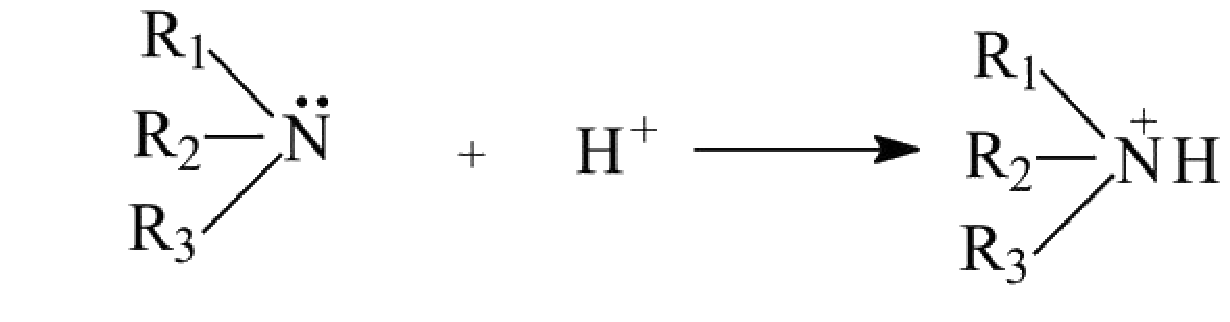
\includegraphics[width=6.0cm]{images_crop_de08/cau03_amine_hplus.png}\par}
Cụm từ điền vào khoảng trống là
\choice
{cho nhận}
{ion}
{cộng hóa trị thường}
{hydrogen}
\loigiai{}
\end{ex}

\begin{ex}
Chất nào sau đây là amino acid?
\choice
{Acid glutaric}
{Acid glutamic}
{Glycerol}
{Aniline}
\loigiai{}
\end{ex}

\begin{ex}
(SBT -- KNTT). Quá trình di chuyển của các amino acid trong điện trường được gọi là
\choice
{sự điện di}
{sự điện li}
{sự điện phân}
{sự điện giải}
\loigiai{}
\end{ex}

\begin{ex}
(SBT -- CTST). Amino acid \textbf{không} có loại phản ứng nào sau đây?
\choice
{Phản ứng với acid và base}
{Phản ứng ester hoá}
{Phản ứng trùng ngưng}
{Phản ứng thủy phân}
\loigiai{}
\end{ex}

\begin{ex}
Số liên kết peptide trong hợp chất pentapeptide là
\choice
{3}
{4}
{5}
{6}
\loigiai{}
\end{ex}

\begin{ex}
(SBT -- KNTT). Loại liên kết được hình thành giữa các amino acid trong peptide được gọi là
\choice
{liên kết ion}
{liên kết hydrogen}
{liên kết peptide}
{liên kết cộng hoá trị}
\loigiai{}
\end{ex}

\begin{ex}
Protein hình cầu tan được trong nước tạo dung dịch keo như
\choice
{$\alpha$-keratin (ở tóc, móng)}
{Collagen (ở da, sụn)}
{Albumin (lòng trắng trứng)}
{Myosin (ở cơ bắp)}
\loigiai{}
\end{ex}

\begin{ex}
Ứng dụng nào sau đây \textbf{không} phải là của protein?
\choice
{Là thành phần tạo nên chất dẻo}
{Là thành phần cấu tạo tế bào}
{Là cơ sở tạo nên sự sống}
{Là dinh dưỡng thức ăn}
\loigiai{}
\end{ex}

\newpage

\begin{ex}
(SBT -- CTST). Trong dãy các chất sau đây, tính base của amine thể hiện qua phản ứng với các chất:
\choice
{\ce{HCl}, \ce{H2SO4}, \ce{CuCl2}}
{\ce{Cl2}, \ce{H2SO4}, \ce{FeCl3}}
{\ce{NaOH}, \ce{HCl}, \ce{FeCl3}}
{\ce{O2}, \ce{HCl}, \ce{CuCl2}}
\loigiai{}
\end{ex}

\begin{ex}
(SBT -- CTST). Cơ thể người mã hoá được loại amino acid nào sau đây trong tổng hợp protein cho cơ thể?
{\centering
	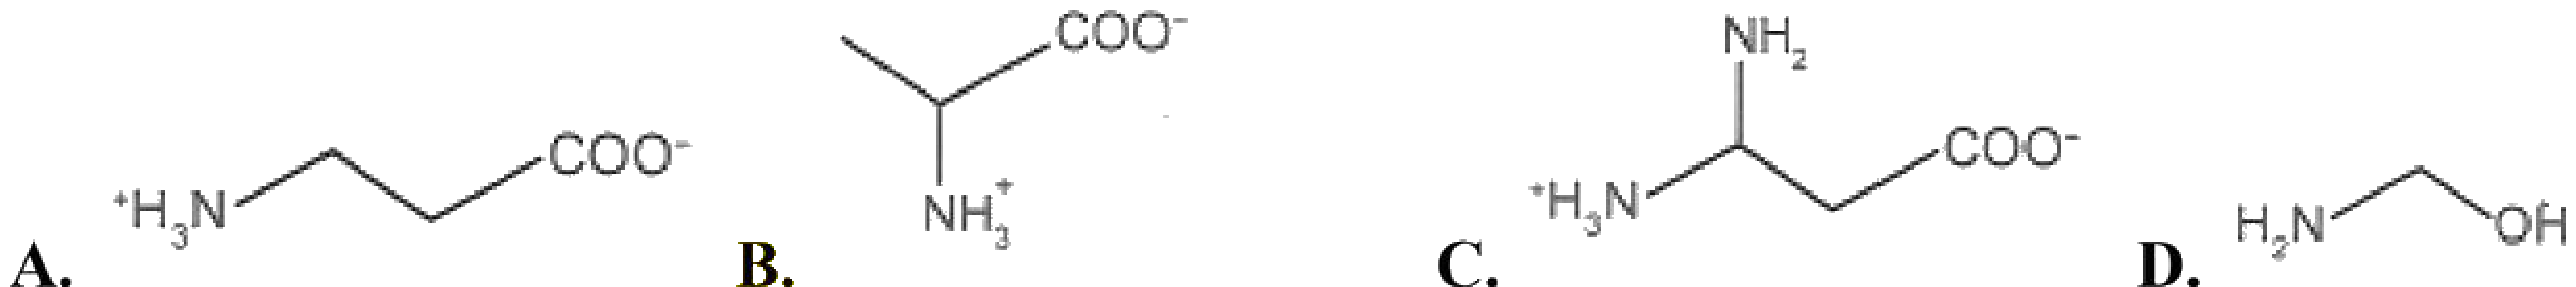
\includegraphics[width=13.5cm]{images_crop_de08/cau12_options.png}\par}
\choice
{Cấu tạo A}
{Cấu tạo B}
{Cấu tạo C}
{Cấu tạo D}
\loigiai{}
\end{ex}

\begin{ex}
(SBT -- KNTT). Trong phản ứng của amine với \ce{Cu(OH)2}, sản phẩm có màu xanh đặc trưng là do
\choice
{sự tạo phức giữa \ce{Cu^2+} và -\ce{NH2}}
{sự oxi hoá \ce{Cu^2+} khi gặp amine}
{phản ứng giữa \ce{OH-} và -\ce{NH2}}
{giải phóng \ce{H2} khi phản ứng}
\loigiai{}
\end{ex}

\begin{ex}
(SBT -- CTST). Cơ thể người sử dụng phân tử nào sau đây để xây dựng protein?
\choice
{Tinh bột}
{Chất béo}
{Amino acid}
{Acid béo}
\loigiai{}
\end{ex}

\begin{ex}
(SBT -- CTST). Các hợp chất amine, amino acid, peptide và protein có nhóm chức chung nào sau đây?
\choice
{Carboxyl}
{Amide}
{Ammonium}
{Amine hoặc amino}
\loigiai{}
\end{ex}

\begin{ex}
Amine và amino acid nào sau đây có cùng bậc?
\choice
{Dimethylamine và alanine}
{Dimethylamine và glutamic acid}
{Dimethylamine và proline}
{Trimethylamine và lysine}
\loigiai{}
\end{ex}

\begin{ex}
(SBT -- CTST). Tính chất hoá học của methylamine và alanine đều có
\choice
{phản ứng với ninhydrin}
{phản ứng thuỷ phân}
{phản ứng với dung dịch \ce{HCl}}
{phản ứng với dung dịch \ce{NaOH}}
\loigiai{}
\end{ex}

\begin{ex}
Cho các phát biểu sau:\\
(a) Trong dung dịch, glycine tồn tại chủ yếu ở dạng ion lưỡng cực.\\
(b) Amino acid là chất rắn kết tinh, dễ tan trong nước.\\
(c) Phản ứng thế bromine vào vòng thơm của aniline dễ hơn benzene.\\
(d) Hợp chất \ce{H2N-CH2-COO-CH3} tác dụng được với dung dịch \ce{NaOH} và dung dịch \ce{HCl}.\\
(e) Triolein và protein có cùng thành phần nguyên tố.\\
(g) Trong phân tử, các amino acid đều chỉ có một nhóm \ce{NH2} và một nhóm \ce{COOH}.\\
Số phát biểu đúng là
\choice
{4}
{5}
{3}
{6}
\loigiai{}
\end{ex}

\Closesolutionfile{ans}

\newpage

\vspace{0.15cm}
\noindent
\textbf{PHẦN II (4,0 điểm -- 4 câu): Câu trắc nghiệm đúng sai.}\\
\textit{Thí sinh trả lời từ câu 1 đến câu 4. Trong mỗi ý a), b), c), d) ở mỗi câu, thí sinh chọn đúng hoặc sai.}

\setcounter{ex}{0}

\begin{ex}
(SBT -- KNTT). Các phát biểu về tính chất hoá học của dung dịch aniline:
\choiceTF
{Dung dịch aniline làm quỳ tím chuyển sang màu xanh}
{Dung dịch aniline tạo kết tủa trắng khi thêm vào nước bromine}
{Aniline phản ứng với \ce{HCl} tạo phenylammonium chloride}
{Aniline phản ứng với \ce{HNO2} tạo muối phenyldiazonium}
\loigiai{}
\end{ex}

\begin{ex}
(SBT -- CTST). Cho một số hợp chất chứa nguyên tố nitrogen như hình bên dưới:\\
{\centering
	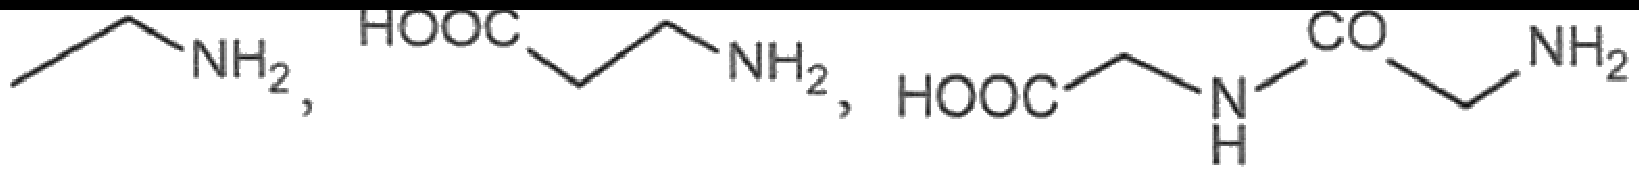
\includegraphics[width=11.5cm]{images_crop_de08/p2_cau2_compounds.png}\par}
Về phân loại hợp chất và đặc điểm cấu tạo, xét tính đúng/sai của các phát biểu sau:
\choiceTF
{Có 1 hợp chất hữu cơ thuộc loại amine}
{Có 2 hợp chất hữu cơ thuộc loại amino acid}
{Có 1 hợp chất hữu cơ đơn chức, 2 hợp chất tạp chức, 3 hợp chất chứa nhóm $\alpha$-\ce{NH2}}
{Trong 3 hợp chất trên chỉ có 1 liên kết peptide}
\loigiai{}
\end{ex}

\begin{ex}
Acetyl Hexapeptide-8 là một hợp chất peptide. Chất này được biết đến là một thành phần có khả năng liên kết với nước để phục hồi da và là một chất dẫn truyền thần kinh làm giảm nếp nhăn hình thành do lão hóa hoặc bởi các biểu hiện thay đổi trên cơ mặt gây ra.
{\centering
	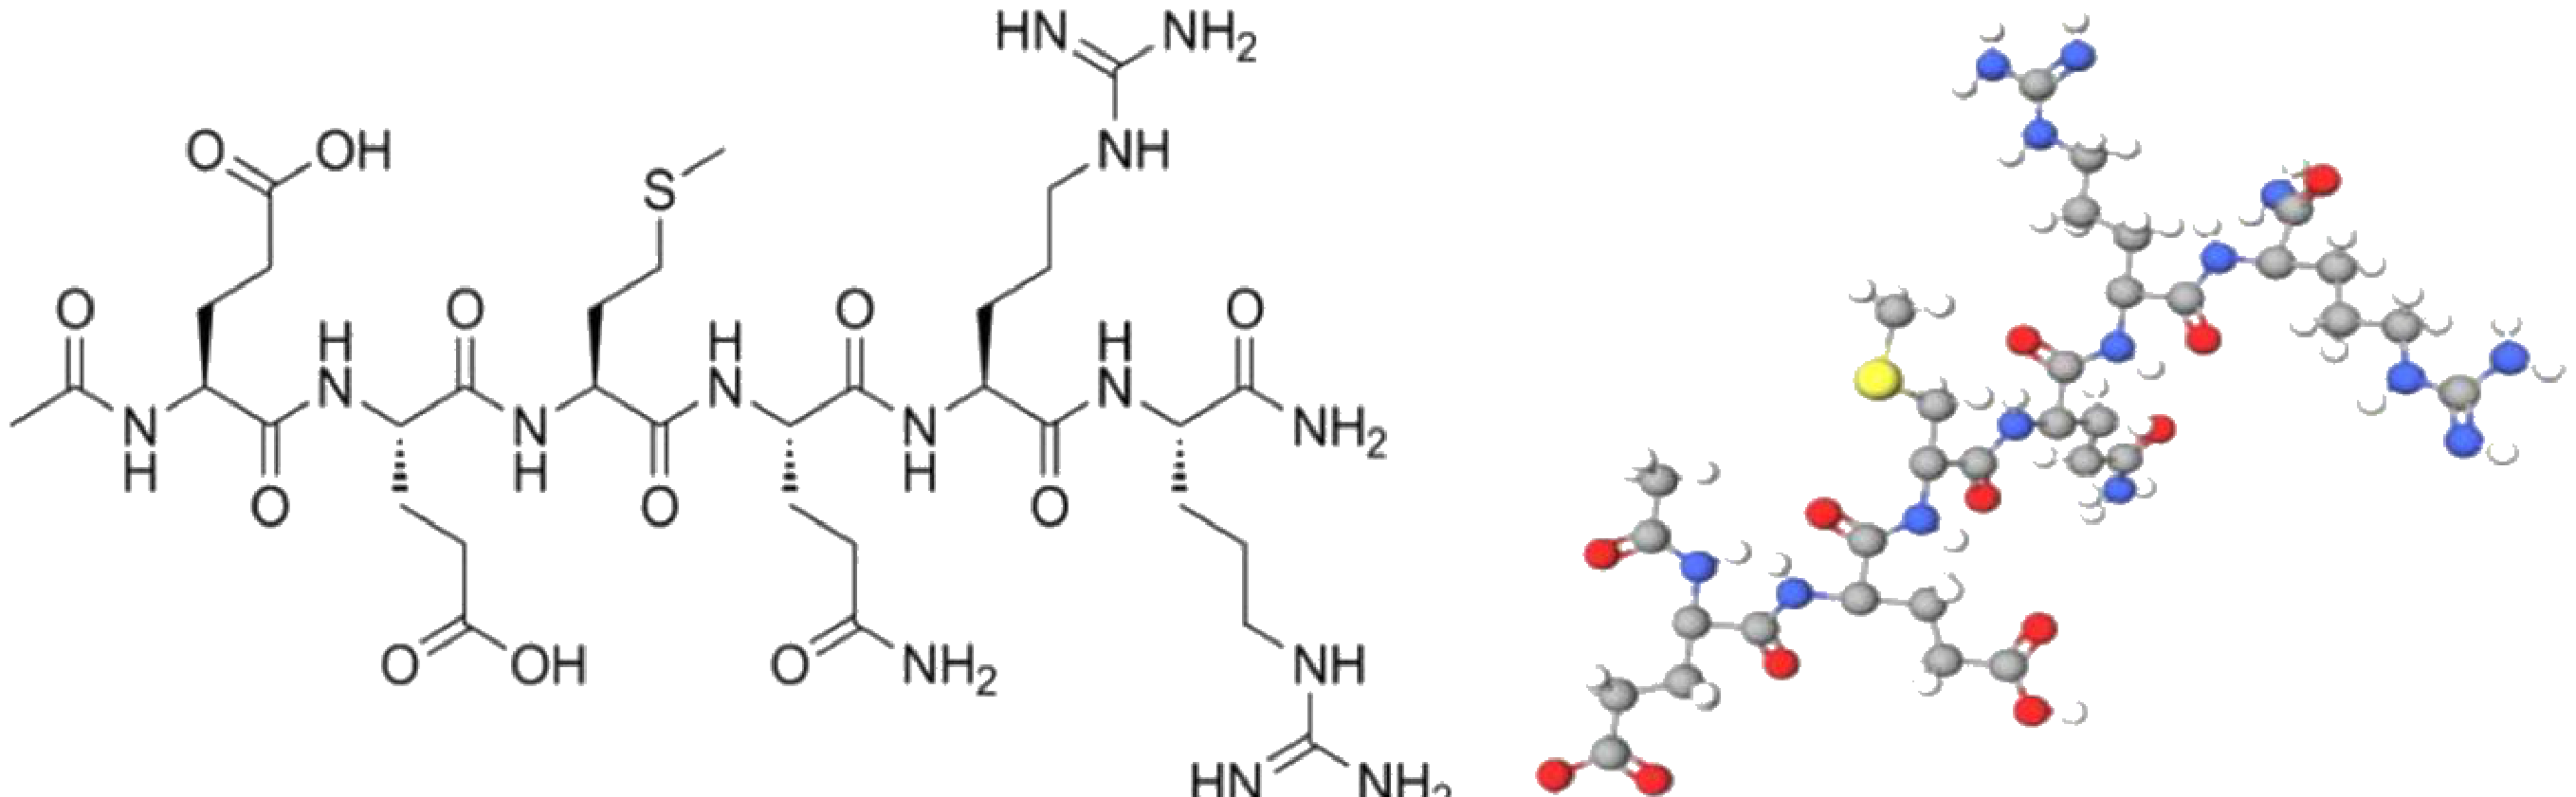
\includegraphics[width=12.5cm]{images_crop_de08/p2_cau3_acetyl_hexapeptide.png}\par}
\choiceTF
{Acetyl Hexapeptide-8 là một hợp chất amino acid}
{Acetyl Hexapeptide-8 có chứa các nguyên tố C, H, N, O}
{Acetyl Hexapeptide-8 là một peptide}
{Acetyl Hexapeptide-8 là một hợp chất tạp chức}
\loigiai{}
\end{ex}

\begin{ex}
Casein là loại protein chủ yếu có trong sữa. Casein là một dạng protein (đạm) có trong sữa mẹ, sữa bò và sữa dê. Vì là protein hoàn chỉnh nên casein bổ sung nhiều amino acid thiết yếu và các hợp chất khác giúp cơ thể tăng trưởng, phát triển.
{\centering
	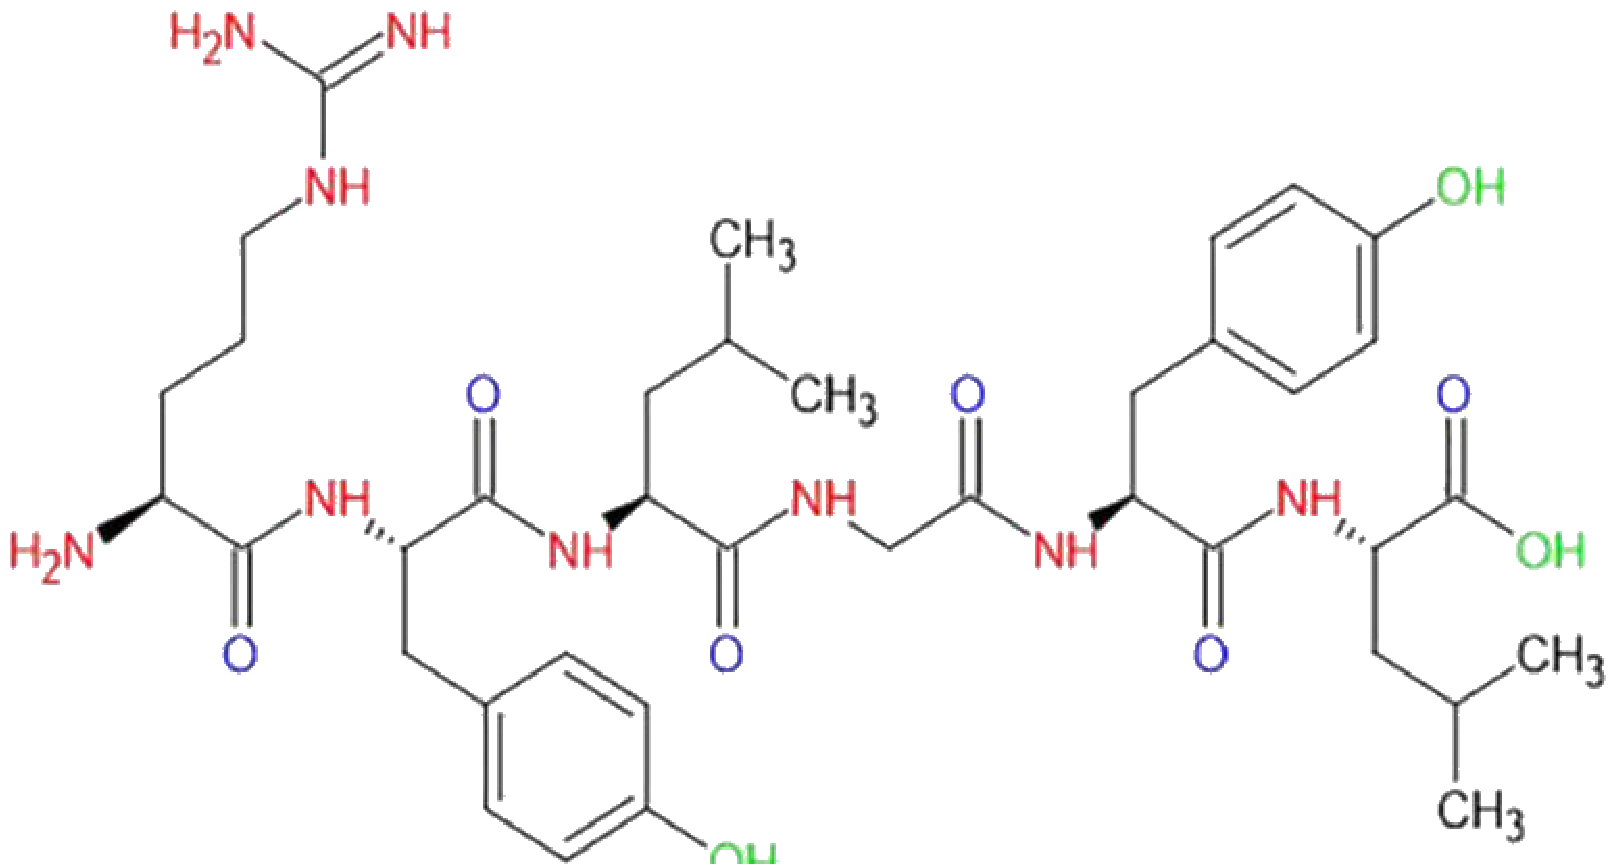
\includegraphics[width=9.5cm]{images_crop_de08/p2_cau4_casein.png}\par}
\choiceTF
{Casein là loại protein tan tốt trong nước}
{Uống sữa giúp giảm bớt nguy hiểm khi bị ngộ độc bởi muối chì, muối thuỷ ngân}
{Vì casein là một loại protein sẽ đông tụ và tách khỏi dung dịch khi thêm dung dịch acid, base, muối của các kim loại nặng như chì, thủy ngân,\dots{} nên uống sữa khi bị ngộ độc muối chì, muối thủy ngân sẽ tạo thành kết tủa và thải được ra ngoài}
{Casein là loại protein có duy nhất trong sữa}
\loigiai{}
\end{ex}

\newpage

\vspace{0.15cm}
\noindent
\textbf{PHẦN III (1,5 điểm -- 6 câu): Câu trắc nghiệm yêu cầu trả lời ngắn.}\\
\textit{Thí sinh trả lời từ câu 1 đến câu 6. Mỗi câu hỏi thí sinh điền câu trả lời vào ô tương ứng.}

\setcounter{ex}{0}

\begin{ex}
Cho ethylamine lần lượt vào dung dịch \ce{FeCl3}; dung dịch \ce{HCl}; \ce{Cu(OH)2}; dung dịch \ce{NaCl}; dung dịch \ce{Br2}. Ethylamine phản ứng được với bao nhiêu chất?
\loigiai{}
\end{ex}
\noindent\textit{Đáp số:} \dotfill\vspace{0.25cm}

\begin{ex}
Cho dãy các dung dịch: acetic acid, phenylammonium chloride, sodium acetate, methylamine, glycine, phenol. Số dung dịch trong dãy tác dụng được với dung dịch \ce{NaOH} là
\loigiai{}
\end{ex}
\noindent\textit{Đáp số:} \dotfill\vspace{0.25cm}

\begin{ex}
Cho các chất: phenylammonium chloride, alanine, lysine, glycine, ethylamine. Số chất làm quỳ tím đổi màu là
\loigiai{}
\end{ex}
\noindent\textit{Đáp số:} \dotfill\vspace{0.25cm}

\begin{ex}
Cho các phát biểu sau:\\
(1) Dung dịch ethylamine và dung dịch aniline đều làm xanh giấy quỳ tím.\\
(2) Nhỏ từ từ đến dư dung dịch methylamine vào dung dịch copper(II) sulfate, ban đầu thấy xuất hiện kết tủa màu xanh nhạt, sau đó kết tủa tan tạo thành dung dịch màu xanh lam.\\
(3) Cho dung dịch methylamine vào ống nghiệm đựng dung dịch iron(III) chloride thấy xuất hiện kết tủa nâu đỏ.\\
(4) Nhỏ vài giọt dung dịch aniline vào ống nghiệm đựng nước bromine thấy xuất hiện kết tủa trắng.\\
Số phát biểu đúng là
\loigiai{}
\end{ex}
\noindent\textit{Đáp số:} \dotfill\vspace{0.25cm}

\begin{ex}
Thuốc Paracetamol là một loại thuốc được sử dụng rất nhiều trong y học. Thuốc có tác dụng giảm đau, hạ sốt tuy nhiên ít có tác dụng kháng viêm. Thuốc Paracetamol được tổng hợp từ p-nitrophenol theo sơ đồ phản ứng sau (biết hiệu suất của cả quá trình phản ứng đạt 90\%):
{\centering
	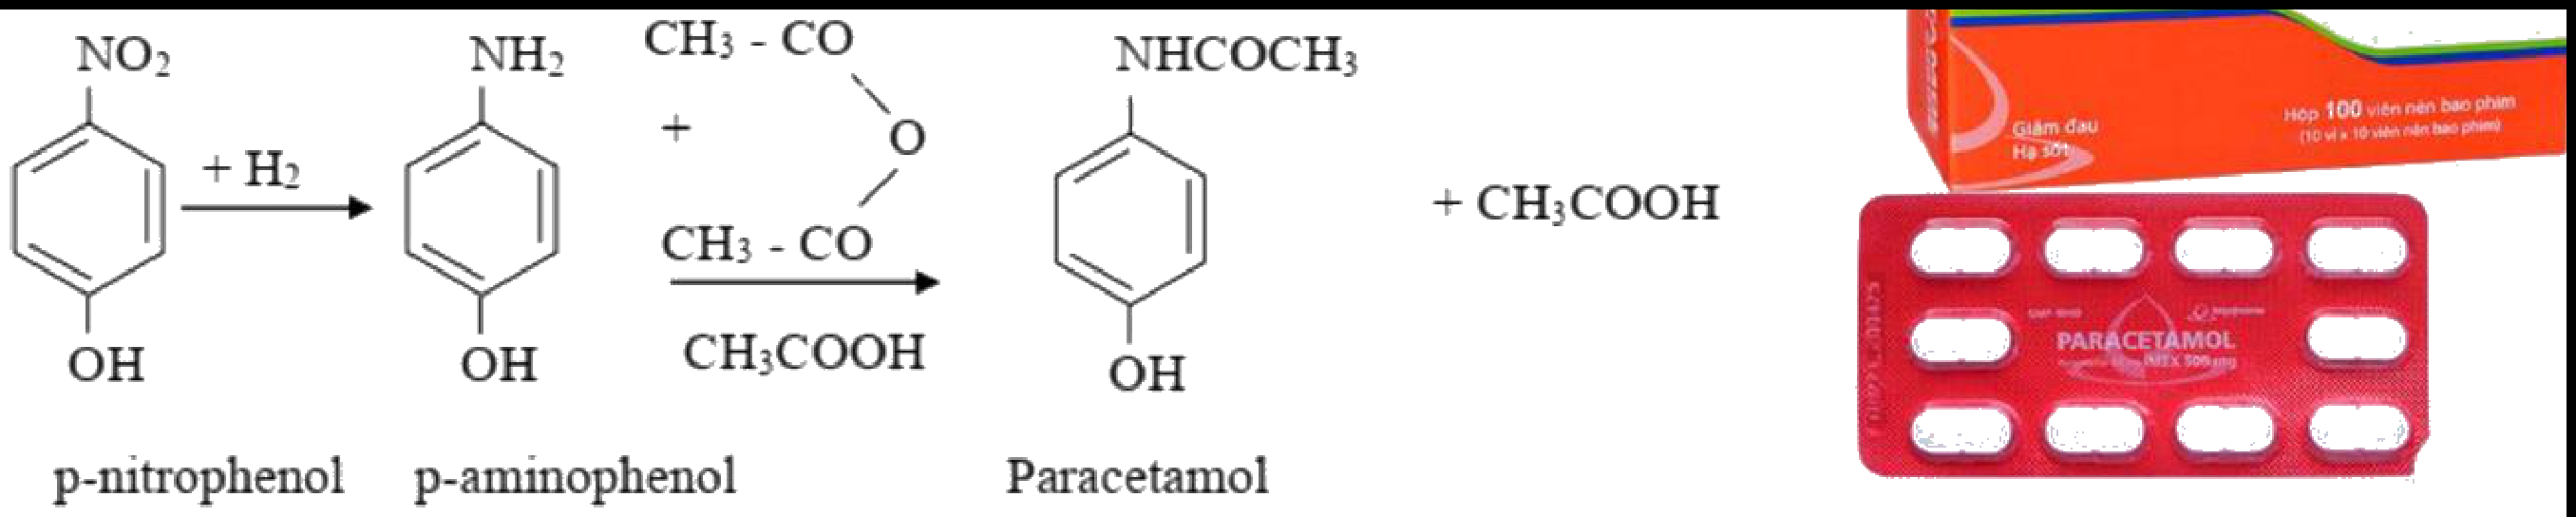
\includegraphics[width=13.0cm]{images_crop_de08/p3_cau5_paracetamol.png}\par}
Để sản xuất 30,2 triệu viên thuốc Paracetamol thì khối lượng p-nitrophenol cần dùng gần nhất với giá trị nào sau đây (theo đơn vị tấn)? Biết rằng mỗi viên thuốc chứa 500 mg Paracetamol.
\loigiai{}
\end{ex}
\noindent\textit{Đáp số:} \dotfill\vspace{0.25cm}

\begin{ex}
Một người trưởng thành cần tiêu thụ khoảng 0,8 gram protein cho mỗi kg trọng lượng cơ thể mỗi ngày. Một người nặng 70 kg cần bổ sung bao nhiêu gram protein trong một ngày? Nếu mỗi quả trứng chứa khoảng 6 gram protein, người đó cần ăn bao nhiêu quả trứng để đáp ứng lượng protein cần thiết trong ngày? Biết số quả trứng là một con số chẵn.
\loigiai{}
\end{ex}
\noindent\textit{Đáp số:} \dotfill\vspace{0.25cm}

\vspace{0.1cm}
\begin{center}
	\textbf{---------- HẾT ----------}
\end{center}

\end{document}
